We next investigate the relationship between segmentation quality and orientation accuracy.
Specifically, we analyze whether higher foreground mIoU correlates with lower orientation errors.

\Cref{fig:iou_vs_orientation_error} shows hexbin plots of foreground mIoU versus absolute orientation error for UNet3 and ResUNet18 on the test set.
A clear negative correlation is evident for both models, as confirmed by Spearman's rank correlation ($\rho = -0.40$, $p < 0.001$ for UNet3 and $-0.73$, $p < 0.001$ for ResUNet18)~\cite{noauthor_nodate_spearmans}: as mIoU increases, orientation error decreases.

However, ResUNet18 predictions are concentrated more tightly in the top left of the plot (high mIoU and low error), while UNet3 predictions are more scattered.
UNet3 produces many examples with low mIoU even when the orientation error is moderate ($\leq$\qty{50}{\degree}), whereas ResUNet18’s predictions are more consistent, with higher mIoU and less variation.

This suggests that better segmentation masks (higher mIoU) generally enable more accurate orientation estimation and that ResUNet18 produces more consistent and reliable segmentations.

We also examined the signed orientation error as a function of the ground-truth angle (see \Cref{fig:appendix_unet3_orientation,fig:appendix_resunet18_orientation}).
No clear dependency was observed; the error distribution appears uniform across the range of ground-truth angles.


\begin{figure}[htbp]
    \centering
    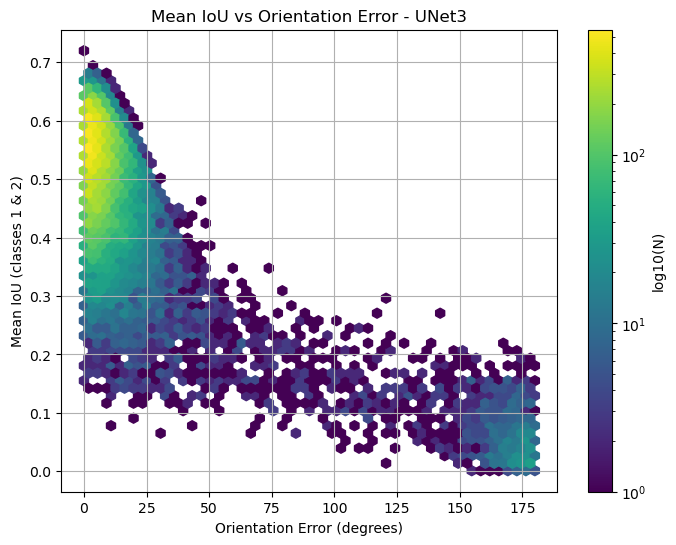
\includegraphics[width=0.49\textwidth]{figures/results/4 - correlation/UNet3 mIoU vs Orientation Error.png}
    \hfill
    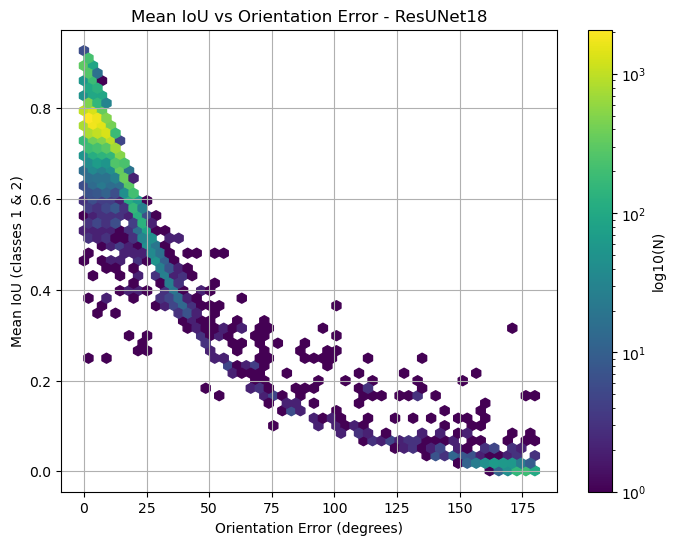
\includegraphics[width=0.49\textwidth]{figures/results/4 - correlation/ResUNet18 mIoU vs Orientation Error.png}
    \caption{
        Hexbin plots of foreground mIoU versus absolute orientation error for (\textbf{left}) UNet3 and (\textbf{right}) ResUNet18.
        Both models exhibit a negative correlation (Spearman’s $\rho = -0.40$ for UNet3, $\rho = -0.73$ for ResUNet18), but ResUNet18 predictions are more concentrated in the upper‑left corner (high mIoU, low error).
        In contrast, UNet3 predictions are dispersed with a broader spread of mIoU for any error.
    }
    \label{fig:iou_vs_orientation_error}
\end{figure}